
\begin{figure}
\begin{center}
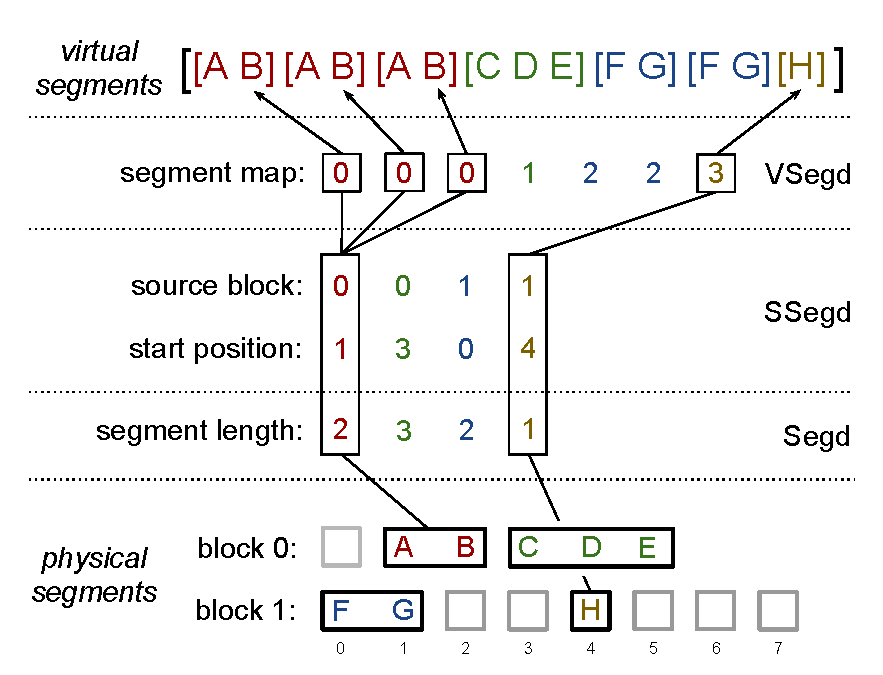
\includegraphics[scale=0.6]{figures/NewArrayRep}
\caption{New Array Representation}
\end{center}
\label{figure:NewArrayPicture}
\end{figure}

\eject{}

% -----------------------------------------------------------------------------
\section{New Representation of Nested Arrays}
\label{section:Segds}

The new array representation must support all index space transforms that vectorisation introduces, in a way that allows the vectorised program to have the same asymptotic complexity as the original unvectorised program. This is up to \emph{containment} which is discussed in \S\ref{section:PackCombine}. In most cases this comes down to having the same complexity as the direct representation, where nested arrays are stored as flat arrays of pointers to more arrays. However, we cannot use this representation as described, because it would lose the granularity and data locality benefits of the baseline segmented representation. We need the best of both worlds.


% -----------------------------------------------------------------------------
\subsection{Physical, Virtual and Scattered Segments}
An example array with the same value as @ARR0@ is shown in Figure~\ref{figure:NewArrayPicture}. Our new representation has the following key features:
\begin{enumerate}
\item   We distinguish between \emph{physical} and \emph{virtual} segments. Physical segments consist of real element data in memory, while virtual segments are defined by mapping onto physical segments. This distinction enables us to define nested arrays with repeated segments without copying element data.

\item   The physical segments of a nested array may now be scattered through several data blocks, instead of being contiguous. Although we prefer segments to be contiguous for locality reasons, we must also allow them to be scattered, so that we can filter a nested array without copying element data.
\end{enumerate}
In the example, there are seven virtual segments defined from four physical segments. The physical segments lie scattered in two data blocks. We will see why we need to allow physical segments to lie in separate data blocks in \S\ref{section:Append}. The overall segment descriptor is now stratified into three layers: @VSegd@ (virtual segments); @SSegd@ (scattered segments) and plain @Segd@ (contiguous segments). In our terminology, we refer to all of @VSegd@, @SSegd@ and @Segd@ as ``segment descriptors'', individually or grouped together. At the bottom layer, @Segd@ gives the length of each segment, and would be sufficient to describe the array if all segments were contiguous in a single block. The @SSegd@ gives the index of the source data block, and starting position for each physical segment in its block. The @VSegd@ provides the mapping between virtual and physical segments. We have elided the @indices@ field from the diagram for clarity, but also include this in our new array representation as part of the @Segd@.


\clearpage{}
% -----------------------------------------------------------------------------
\subsection{The Concrete Definition}
\label{section:Representation}

\begin{figure}
\begin{small}
\begin{code}
data PA e = PA { length :: Int, pdata :: PData e }
data family   PData  e
data family   PDatas e
data instance PData  Int  = PInt   (Vector Int)
data instance PDatas Int  = PInts  (Vector (Vector Int))
data instance PData  Char = PChar  (Vector Char)
data instance PDatas Char = PChars (Vector (Vector Char))

data instance PData (PA e)
 = PNested { vsegd :: VSegd, pdatas :: PDatas e }

data instance PDatas (PA e)
 = PNesteds (Vector (PData (PA e)))

data VSegd  -- Virtual-segment descriptor.
 = VSegd { segmap  :: Vector PsId, ssegd :: SSegd }

data SSegd  -- Scattered-segment descriptor.
 = SSegd { sources :: Vector DbId, starts :: Vector Int }
         , segd    :: Segd }

data Segd   -- Contiguous-segment descriptor.
 = Segd  { lengths :: Vector Int, indices :: Vector Int }

type PsId = Int  -- Physical segment Id, indexes 'sources'
type DbId = Int  -- Data block Id, indexes 'pdatas'
\end{code}
\end{small}
\caption{Definition of the New Array Representation}
\label{figure:NewArrayRepresentation}
\end{figure}

The concrete definition of our new array type is given in Figure~\ref{figure:NewArrayRepresentation}. The data type @PA@ is unchanged from Figure~\ref{figure:OldArrayRepresentation}: a pair of a length and payload. The instances for @PData Int@ and @PData Char@ are also unchanged. The difference is in the representation of nested arrays:
\begin{small}
\begin{code}
  data instance PData (PA a)
   = PNested { vsegd  :: VSegd, pdatas :: PDatas a }
\end{code}
\end{small}
The payload is now a @PDatas@ (plural) rather than @PData@. Where @PData@ represents a single data block, @PDatas@ represents a vector of data blocks. We use the type @DbId@ (short for data-block identifier) to index this vector of @PData@ values. 

The @vsegd@ field holds the \emph{virtual segment descriptor}.  It consists of a vector of physical segment identifiers (@segmap@), and a scattered segment descriptor (@ssegd@). The @segmap@ maps virtual segments onto physical segments and corresponds 1-1 with the outer level of the array being represented. In Figure~\ref{figure:NewArrayPicture}, we have seven entries in this map and seven subarrays in the overall nested array.

Each entry in the @segmap@ is a \emph{physical segment identifier}, of type @PsId@. A @PsId@ is the index of one of
the physical segments described by the @SSegd@ and @Segd@ types. Crucially, the @segmap@ can contain repeated use of the same physical segment. In Figure~\ref{figure:NewArrayPicture} we have used @[0 0 0 1 2 2 3]@ to indicate three copies of the first physical segment, one copy of the second, and so on. This is how we represent the sharing defined by @replicates@. Note that we can not just store the replication counts @[3 1 2 1]@ directly because we must be able to map virtual segments to physical segments in constant time.

The @SSegd@ and @Segd@ together describe the physical segments. Together they contain four vectors, \emph{all of the same length}, two of them nested inside the @segd@ field. The @sources@ vector gives the data block identifier, @DbId@, which is the index of one of the data blocks in the @pdatas@ field. The next two, @starts@ and @lengths@, give the starting position and length of the physical segment in that data block. Finally @indices@ is, as before, a cached copy of the scan (accumuated sum) of @lengths@. Keeping @SSegd@ and @Segd@ separate is helpful when optimising vectorised code for absolute performance, which we discuss in \S\ref{section:Pragmatics}. 

Finally, the array representation must obey the following invariants:

\begin{enumerate}
\item	The lengths of the @sources@, @starts@, @lengths@, and @indices@ fields must all be the same.

\item	Every @PsId@ in the @segmap@ must be less than the length of the @sources@ field. 

\item	Each @DbId@ in @sources@ must be less than the length of the @pdatas@ vector.

\item	Each element of @starts[i]@ must be less than the length of @pdatas[sources[i]]@.

\item	The @indices@ field is equal to @init (scan (+) 0 lengths)@.

\item	All physical segments defined by the @SSegd@ and @Segd@ types must be reachable from the @segmap@. More precisely, the set of physical segment identifiers in the @segmap@ must cover @[0..np-1]@, where @np@ is the length of the @starts@, @sources@, @lengths@, and @indices@ fields.

\item	All @pdata@ blocks must be reachable from the @sources@ field.  More precisely, the set of @sources@ must cover @[0..nb-1]@, where @nb@ is the length of the @pdatas@ vector.
\end{enumerate}

Invariants 1 to 4 are standard well-formedness conditions. Invariant 2 ensures that each physical segment identifier points to a real physical segment. Invariant 3 ensures that each data block identifier points to a real data block. Invariant 5 says that @indices@ is precomputed from @lengths@. The reason for this is discussed in \S\ref{section:Pragmatics}. Invariants 6 and 7 ensure that the size of the internal structure of the array is bounded by the number of virtual segments, which is necessary for the complexity bound on @append@ (\S\ref{section:Append}). Invariant 7 is also needed to ensure that the parallel implementation of reductions such as @sum@ do not duplicate work (\S\ref{section:Reduction}). However, an implementation may be able to relax these last two invariants in certain cases (\S\ref{section:Pragmatics}).


% -----------------------------------------------------------------------------
\subsection{Replicates again}
\label{section:Replicates}
Now let us implement @replicates@ using our new array representation. The start is easy, because the result @PA@ array must be built with a @PA@ constructor:
\par
\begin{small}
\begin{code}
 replicates :: Vector Int -> PA e -> PA e
 replicates ns arr = PA (sum ns) (replicatesPR ns arr)
\end{code}
\end{small}
\par
\noindent
The real work is in @replicatesPR@.  But now we encounter a slight problem: since the representation of @PData@ is indexed by the element type @e@, we require a type-indexed function to operate over @PData@ values.  That is, we need a type class, with an instance for @Int@ and an instance for @(PA e)@:
\begin{small}
\begin{code}
 class PR e where
   replicatesPR :: Vector Int -> PData e -> PData e
   ...more methods...

 instance PR Int where
   replicatesPR = replicatesI
   ...
 instance PR e => PR (PA e) where
   replicatesPR = replicatesPA
   ...
\end{code}
\end{small}
The @PR@ (Parallel Representation) class is given in Figure \ref{figure:NewArrayOperators}, and conveniently collects all the necessary primitive operations over arrays.  We will see more of them in this section, but @replicatesPR@ is one. So, in fact, we lied: the types of @replicates@ and @replicatesPR@ are overloaded thus:
\par
%
\begin{small}
\begin{code}
 replicates   :: PR e => Vector Int -> PA e    -> PA e
 replicatesPR :: PR e => Vector Int -> PData e -> PData e
\end{code}
\end{small}
\par
\begin{figure}
\begin{small}
\begin{code}
class PR e where
emptyPR      :: PData  e
lengthPR     :: PData  e -> Int                                   

replicatePR  :: Int        -> e       -> PData e
replicatesPR :: Vector Int -> PData e -> PData e

appendPR     :: PData  e -> PData e -> PData e

indexPR      :: PData  e -> Int -> e                              
indexvsPR    :: PDatas e -> VSegd 
             -> Vector (Int, Int) -> PData e

extractPR    :: PData  e -> Int   -> Int -> PData e
extractvsPR  :: PDatas e -> VSegd -> PData e

packPR   :: PData  e -> Vector Bool -> PData e
combinePR:: Vector Bool -> PData e -> PData e -> PData e

lengthdPR    :: PDatas e -> Int
emptydPR     :: PDatas e
singletondPR :: PData  e -> PDatas e
appenddPR    :: PDatas e -> PDatas e -> PDatas e
indexdPR     :: PDatas e -> Int -> PData e

------- Utility functions --------
sumV        :: Vector Int -> Int
singletonV  :: e -> Vector e
replicateV  :: Int -> e -> Vector e
replicatesV :: Vector Int -> Vector e -> Vector e
\end{code}
\end{small}
\caption{Primitive Array Operators}
\label{figure:NewArrayOperators}
\end{figure}
%
\noindent
(In what follows we will often omit the ``@PR =>@'' context from types to save space.)
Now we are ready to implement the two cases.
The case for @Int@ is straightforward:
\par
\begin{small}
\begin{code}
 replicatesI :: Vector Int -> PData Int -> PData Int
 replicatesI ns (PInt xs) = PInt (replicatesV ns xs)
\end{code}
\end{small}
\par
\noindent
where @replicatesV@ is the @Vector@-level replication operation shown in Figure~\ref{figure:NewArrayOperators}. The interesting case is the one for nested arrays:
\par
\begin{small}
\begin{code}
 instance PR e => PR (PA e) where
  replicatesPR = replicatesPA

 replicatesPA :: Vector Int -> PData (PA e) -> PData (PA e)
 replicatesPA lens (PNested segmap pdatas)
  = PNested (VSegd segmap' ssegd) pdatas
  where segmap' = replicatesV lens segmap
\end{code}
\end{small}
\par
With our new array representation, we can apply segmented replicate to an array by using @replicatesV@ on the @segmap@ field. The element data, @pdatas@, does not need to be copied, and is untouched in the result. Continuing the example from \S\ref{section:naive-flat}, applying @replicates@ to the array from Figure~\ref{figure:NewArrayPicture} yields:
\par
\begin{small}
\begin{code}
   replicates [0 0 1 1 0 0 1] {Figure 3}
 = [[A B] [C D E] [H]]
 ------------------------------------------------ (ARR1)
  PA 3 (PNested
   (VSegd  segmap: [0 1 3]
   (SSegd sources: [0 0 1 1]  starts: [1 3 0 4])
   (Segd  lengths: [2 3 2 1] indices: [0 2 5 7]))
   (PChars 0: [X A B C D E]
           1: [F G X X H X X X])
\end{code}
\end{small}
\par
In fact, the above definition of @replicatesPA@ function is not yet complete. Physical segments 0, 1 and 3 are used, but segment 2 is not, which violates invariant 6. We will discuss why this matters in \S\ref{section:Culling}.


% -----------------------------------------------------------------------------
\subsection{Plain replicate}
\label{section:PlainReplicate}
\noindent
Vectorisation also uses a simpler form of replication, which we call @replicate@ (singular). The call @(replicate n x)@ returns an array of @n@ elements, each a (virtual) copy of @x@. This function is introduced when an inner parallel computation uses a shared constant or a free variable that is defined in an outer context. This is essentially the same reason that the more general @replicates@ function is introduced, though with plain @replicate@ the shared value is used uniformly by all inner computations. We will see an example in \S\ref{section:RewriteRules}. Note that unlike @replicates@, the result of plain @replicate@ has a greater nesting depth than the source element. The interesting case is for nested arrays:
%
\begin{small}
\begin{code}
 replicatePA :: Int -> PA e -> PData (PA e)
 replicatePA c (PA n pdata)
  = replicatesPR (singletonV c) 
  $ PNested (singletonVSegd n) (singletondPR pdata)

 singletonVSegd :: Int -> VSegd
 singletonVSegd len
  = VSegd (singletonV 0)
   (SSegd (singletonV 0)   (singletonV 0)
   (Segd  (singletonV len) (singletonV 0)))
\end{code}
\end{small}
%
\noindent
To perform a @replicate@ we simply add a new segment descriptor on top of the old array. This furnishes us with an example array of greater nesting depth:
%
\begin{small}
\begin{code}
  replicate 2 {Figure 3}
 ------------------------------------------------ (ARR2)
  PA 2 (PNested
   (VSegd  segmap: [0 0] 
   (SSegd sources: [0]  starts: [0]
   (Segd  lengths: [7] indices: [0])))
   (PNesteds 
    0: PNested
       (VSegd  segmap: [0 0 0 1 2 2 3]
       (SSegd sources: [0 0 1 1]  starts: [1 3 0 4])
       (Segd  lengths: [2 3 2 1] indices: [0 2 5 7]))
       (PChars 0: [X A B C D E]
               1: [F G X X H X X X])
\end{code}
\end{small}

Notice that the cost of @(replicate n x)@ is $O(@n@)$, regardless of how much data @x@ contains. With our new representation the complexity of @replicate@ is linear in the length of the created @segmap@, which is also the length of the overall array. 


% -----------------------------------------------------------------------------
\subsection{Append} 
\label{section:Append}
Let us consider another important operation: appending two arrays.
\begin{small}
\begin{code}
  appendPA :: PA e -> PA e -> PA e
\end{code}
\end{small}
As mentioned in \S\ref{section:Representation} we need invariants 6 and 7 to achieve the Complexity Goal here. Append should be linear in the length of the two argument arrays, regardless of how deeply nested they are. This is impossible with the baseline representation from \S\ref{section:naive-flat} because we would need to copy all elements into a single data block. 

With our new representation we do not need to copy array elements. To append two nested arrays we append the two @PDatas@ and combine the segment descriptor fields. Although we can simply append the @lengths@ and @starts@ fields, we need to recompute the @indices@. We also need to increment the entries in the second @segmap@ and @sources@ field to account for the physical segments and data blocks defined by the first array. For this process to have complexity linear in the length of the two argument arrays, the lengths of their @starts@, @sources@, @lengths@ and @indices@ fields can be no greater than the length of their @segmap@. To put this another way: the number of physical segments can be no greater than the number of virtual segments. Likewise, the length of the two @PDatas@ can be no greater than the @sources@ fields. These constraints are implied by invariants 6 and 7. The definition of @appendPR@ (the version that works on @PData@) is on the next page.

\clearpage{}
\begin{small}
\begin{code}
appendPR :: PData (PA e) -> PData (PA e) -> PData (PA e)
appendPR (PNested vsegd1 pds1) (PNested vsegd2 pds2)
  = PNested (appendVSegd (length pds1) vsegd1 vsegd2)
            (pds1 ++ pds2) 

appendVSegd ps1 (VSegd sm1 ssegd1) (VSegd sm2 ssegd2)
  = VSegd (sm1 ++ map (+ lengthSSegd ssegd1) sm2)
  $ appendSSegd ps1 ssegd1 ssegd2

appendSSegd ps1 (SSegd ss1 us1 segd1) (SSegd ss2 us2 segd2)
  = SSegd (ss1 ++ ss2) (us1 ++ map (+ ps1) us2)
  $ appendSegd segd1 segd2

appendSegd (Segd ls1 is1) (Segd ls2 is2)
  = let n1 = sum ls1
    in  Segd  (ls1 ++ ls2) (is1 ++ map (+ n1) is2)
\end{code}
\end{small}
\noindent
Here is an example array that we will use in a moment:
\par
\begin{small}
\begin{code}
                 [[K] [] [L M N O]]
------------------------------------------------- (ARR3)
PA 3 (PNested
(VSegd  segmap: [0 1 2]
(SSegd sources: [0 0 0] starts:  [0 1 1])
(Segd  lengths: [1 0 4] indices: [0 1 1]))
(PChars 0: [K L M N O]))
\end{code}
\end{small}
\par
\noindent
Appending the array from Figure~\ref{figure:NewArrayPicture} with @ARR3@ above yields:
\par
\begin{small}
\begin{code}
   [[A B] [A B] [A B] [C D E] ...  [K] [] [L M N O]
------------------------------------------------- (ARR4)
PA 10 (PNested
(VSegd  segmap: [0 0 0 1 2 2 3 4 5 6]
(SSegd sources: [0 0 1 1 2 2 2]  starts: [1 3 0 4 0 1 1] 
(Segd  lengths: [2 3 2 1 1 0 4] indices: [0 2 5 7 8 9 9])))
(PChars 0: [X A B C D E] 
        1: [F G X X H X X X]
        2: [K L M N O]))
\end{code}
\end{small}
%
The data block of @ARR3@ joins the set of data blocks in the result without any copying.

% -----------------------------------------------------------------------------
\subsection{Culling Physical Segments}
\label{section:Culling}
As mentioned in \S\ref{section:Append}, we need invariants 6 and 7 to ensure that @appendPA@ has the correct asymptotic complexity. Suppose we wish to append @ARR1@ from \S\ref{section:Replicates} to @ARR3@ above. Invariant 7 is already satisfied, so this part is fine. However, as we produced @ARR1@ by using a @replicates@ operation with zero valued replication counts, physical segment 2 is no longer reachable from the @segmap@, which violates invariant 6. To recover this we use the following operations:
\par
\begin{small}
\begin{code}
cullOnSegmap::Vector PsId-> SSegd-> (Vector PsId, SSegd)
cullOnSSegd ::   SSegd   -> PDatas e-> (SSegd, PDatas e)
\end{code}
\end{small}
\par
The @cullOnSegmap@ function takes the @segmap@ and @SSegd@ for an array. It filters out the physical segments from the @SSegd@ that are unreachable from the @segmap@, returning an updated @segmap@ and @SSegd@. In the result, the number of physical segments is necessarily bounded by the length of @segmap@. Likewise, @cullOnSSegd@ filters out data blocks in the @PDatas@ not reachable from the @sources@ field of the @SSegd@. We need this second operation because performing just the first could leave some data blocks unreachable from the @sources@ field, thus violating invariant 7. Culling @ARR1@ yields:
\par
\begin{small}
\begin{code}
              [[A B] [C D E] [H]]
 ------------------------------------------------ (ARR5)
  PA 3 (PNested
   (VSegd  segmap: [0 1 2]
   (SSegd sources: [0 0 1]  starts: [1 3 4])
   (Segd  lengths: [2 3 1] indices: [0 2 5]))
   (PChars 0: [X A B C D E]
           1: [F G X X H X X X])
\end{code}
\end{small}
\par
All array operators that filter out entries from the @segmap@ need to apply @cullOnSegmap@ and @cullOnSSegd@ to preserve the invariants. For example, the invariant preserving version of @replicatesPA@ is as follows:
\par
\begin{small}
\begin{code}
replicatesPA:: Vector Int -> PData (PA e) -> PData (PA e)
replicatesPA lens (PNested (VSegd segmap ssegd) pdatas)
 = PNested (VSegd segmap' ssegd'') pdatas'
 where (segmap', ssegd') 
        = cullOnSegmap (replicatesV lens segmap) ssegd
       (ssegd'',  pdatas')
        = cullOnSSegd   ssegd' pdatas
\end{code}
\end{small}
\par
%\simon{At first it all seems totally straightforward.  But the point is that we need a data-parallel implementation, isn't it?  Indeed we should somewhere point out that all operations on segment vectors must be deta-parallel; they look short in the examples, but in fact they can be as big as the data arrays!}
We will now sketch how @cullOnSegmap@ is implemented, leaving the full details to the companion technical report~\cite{lippmeier-etal:replicate-tr}.  The operation of @cullOnSSegd@ is similar. We start by producing a vector of flags that record which of the physical segments are reachable from the @segmap@. For @ARR1@ this is @[T T F T]@. The flags are calculated by first filling the target vector with the default value @F@ and then using \emph{concurrent writes} to set elements referenced by the @segmap@ to @T@. Then, we use the flags vector to compute the physical segment identifiers that appear in the result: @[0 1 3]@. We expand this vector to one that maps between the physical segment identifiers in the result to the identifiers in the source: @[0 1 X 2]@. The @X@ indicates an unused element, which the implementation can fill with any value. Finally, we use this mapping to permute the @segmap@, @sources@, @starts@ and @lengths@ fields of the source array, and then recompute the @indices@.

The work and space complexity of @cullOnSegmap@ is linear in the length of the @segmap@ being processed and the number of physical segments referenced. Likewise, the complexity of @cullOnSSegd@ is linear in the length of the @SSegd@ and the number of data blocks. This ensures that we do not break the complexity budget of operations such as @replicates@ that make use of these functions.


